\chapter{Specifikacija programske potpore}
		
	\section{Funkcionalni zahtjevi}
		
		
		
		\noindent \textbf{Dionici:}
		
		\begin{packed_enum}
			
			\item Ponuđač
			\item Kupac			
			\item Administrator
			
		\end{packed_enum}
		
		\noindent \textbf{Aktori i njihovi funkcionalni zahtjevi:}
		
		
		\begin{packed_enum}
			\item  \underbar{Neregistrirani/neprijavljeni korisnik (inicijator) može:}
			
			\begin{packed_enum}
				
				\item pregledavati i pretraživati oglase
				\item pregledavati statistike oglasa
				
			\end{packed_enum}
			
			\item  \underbar{Registrirani kupac (inicijator) može:}
			
			\begin{packed_enum}
				
				\item pregledavati i pretraživati oglase
				\item kontaktirati ponuđača vezano za oglas
				\item rezervirati oglas
				\item otkazati rezervaciju oglasa
				\item pregledavati i uređivati osnovne podatake
				\item pregledavati i slati poruke
				\item pregledavati kupljene oglase
				
			\end{packed_enum}
			
			\item \underbar{Registrirani ponuđač (inicijator) može:}
			
			\begin{packed_enum}
				\item pregledavati i pretraživati oglase 
				\item kontaktirati ponuđača vezano za oglas
				\item rezervirati oglas
				\item otkazati rezervaciju oglasa
				\item pregledavati i uređivati osnovne podatke
				\item pregledavati i slati poruke
				\item pregledavati kupljene oglase
				\item objavljivati oglase
				\item brisati i uređivati vlastite oglase
				\item potvrditi preuzimanje/prodaju
				
			\end{packed_enum}
			
			\item \underbar{Administrator (inicijator) može:}
			
			\begin{packed_enum}
				\item pregledavati i pretraživati oglase
				\item kontaktirati ponuđača vezano za oglas
				\item rezervirati oglas
				\item otkazati rezervaciju oglasa
				\item pregledavati i uređivati osnovne podatake
				\item pregledavati i slati poruke svim korisnicima
				\item pregledavati vlastite kupljene oglase
				\item vidjeti popis svih registriranih korisnika i njihovih podataka
				\item brisati oglase
				\item privremeno ili trajno blokirati ostale korisnike
				
			\end{packed_enum}
			
			\item \underbar{Baza podataka (sudionik):}
			
			\begin{packed_enum}
				\item pohranjuje sve podatke o korisnicima i njihovim ovlastima
				\item pohranjuje sve podatke o oglasima
				
				
			\end{packed_enum}
		\end{packed_enum}
		
		\eject 
			
				
			\subsection{Obrasci uporabe}
				
			
				
				\subsubsection{Opis obrazaca uporabe}
					

					\noindent \underbar{\textbf{UC1 - Pregled oglasa}}
					\begin{packed_item}
						
						\item \textbf{Glavni sudionik: } korisnik, kupac
						\item  \textbf{Cilj:} Pregledati oglase
						\item  \textbf{Sudionici:} Baza podataka
						\item  \textbf{Preduvjet:} -
						\item  \textbf{Opis osnovnog tijeka:}
						
						\item[] \begin{packed_enum}
							
							\item Karta je prikazana prilikom učitavanja aplikacije
							\item Korisnik dopušta pristup lokaciji i potvrđuje njezinu ispravnost
							\item Prikazuju se oglasi u blizini korisnika
							\item Odabirom oglasa se prikazuju informacije o oglasu
						\end{packed_enum}
						
						\item  \textbf{Opis mogućih odstupanja:}
						
						\item[] \begin{packed_item}
							
							\item[2.a] Korisnik ne dopušta pristup lokaciji 
							\item[] \begin{packed_enum}
								
								\item Korisniku ponuditi mogućnost ručnog unosa lokacije
								\item Korisniku omogućiti pregledavanje oglasa bez unosa lokacije
								
							\end{packed_enum}
							\item[2.b] Automatski određena lokacija je neprecizna
							\item[] \begin{packed_enum}
								
								\item Korisniku ponuditi mogućnost ručnog unosa lokacije
								
							\end{packed_enum}
							
						\end{packed_item}
					\end{packed_item}
					
					\noindent \underbar{\textbf{UC2 - Registracija}}
					\begin{packed_item}
						
						\item \textbf{Glavni sudionik: } Korisnik 
						\item  \textbf{Cilj:} Stvoriti korisnički račun za pristup sustavu
						\item  \textbf{Sudionici:} Baza podataka
						\item  \textbf{Preduvjet:} -
						\item  \textbf{Opis osnovnog tijeka:}
						
						\item[] \begin{packed_enum}
							
							\item Korisnik odabire opciju za registraciju
							\item Korisnik unosi korisničke podatke
							\item Korisnik prima obavijest o uspješnoj registraciji
							
						\end{packed_enum}
						
						\item  \textbf{Opis mogućih odstupanja:}
						
						\item[] \begin{packed_item}
							
							\item[2.a] Odabir već zauzetog korisničkog imena i/ili e-maila, unos korisničkog
							podatka u nedozvoljenom formatu ili pružanje neispravnoga e-maila
							\item[] \begin{packed_enum}
								
								\item Sustav obavještava korisnika o neuspjelom upisu i vraća ga na stranicu za registraciju
								\item Korisnik mijenja potrebne podatke te završava unos ili odustaje od
								registracije
								
							\end{packed_enum}
							
						\end{packed_item}
					\end{packed_item}
					
					\noindent \underbar{\textbf{UC3 - Prijava u sustav}}
					\begin{packed_item}
						
						\item \textbf{Glavni sudionik: } Kupac
						\item  \textbf{Cilj:} Dobiti pristup dodtanim mogućnostima registriranog kupca
						\item  \textbf{Sudionici:} Baza podataka
						\item  \textbf{Preduvjet:} Registracija
						\item  \textbf{Opis osnovnog tijeka:} 
						
						\item[] \begin{packed_enum}
							
							\item Unos korisničkog imena i lozinke
							\item Potvrda o ispravnosti unesenih podataka
							\item Pristup korisničkim funkcijama
						\end{packed_enum}
						
						\item  \textbf{Opis mogućih odstupanja:}
						
						\item[] \begin{packed_item}
							
							\item[2.a] Neispravno korisničko ime/lozinka
							\item[] \begin{packed_enum}
								
								\item Sustav obavještava korisnika o neuspjelom upisu, savjetuje da provjeri podatke i ponovno pokuša ili ako nema račun ga navodi na registraciju
								
							\end{packed_enum}
							
						\end{packed_item}
					\end{packed_item}
					
					\noindent \underbar{\textbf{UC4 - Pregled osobnih podataka}}
					\begin{packed_item}
						
						\item \textbf{Glavni sudionik: } Kupac/ponuđač
						\item  \textbf{Cilj:} Pregledati osobne podatke
						\item  \textbf{Sudionici:} Baza podataka
						\item  \textbf{Preduvjet:} Prijava
						\item  \textbf{Opis osnovnog tijeka:}
						
						\item[] \begin{packed_enum}
							
							\item Korisnik odabire opciju "Osobni podatci"
							\item Aplikacija prkazuje osobne podatke korisnika
							
							
							
						\end{packed_enum}
					\end{packed_item}
					
					\noindent \underbar{\textbf{UC5 - Promjena osobnih podataka}}
					\begin{packed_item}
						
						\item \textbf{Glavni sudionik: } Kupac
						\item  \textbf{Cilj:} Promijeniti osobne podatke
						\item  \textbf{Sudionici:} Baza podataka
						\item  \textbf{Preduvjet:} Prijava
						\item  \textbf{Opis osnovnog tijeka:} 
						
						\item[] \begin{packed_enum}
							
							\item Korisnik odabire opciju uređivanja određenog osobnog podatka
							\item Korisnik mijenja osobni podatak
							\item Korisnik sprema promjene
							\item Baza podataka se ažurira
							\item Korisnik prima potvrdu promjene osobnih podataka
						\end{packed_enum}
						
						\item  \textbf{Opis mogućih odstupanja:}
						
						\item[] \begin{packed_item}
							
							\item[2.a] Korisnik promijeni svoje osobne podatke, ali ne odabere opciju ”Spremi promjenu”
							\item[] \begin{packed_enum}
								
								\item Sustav obavještava korisnika da nije spremio podatke prije izlaska
								iz prozora
								
							\end{packed_enum}
							\item[3.a] Odabir već zauzetog korisničkog imena i/ili e-maila, unos korisničkog
							podatka u nedozvoljenom formatu ili pružanje neispravnoga e-maila
							\item[] \begin{packed_enum}
								
								\item Sustav obavještava korisnika o neuspjelom spremanju i ističe problematične podatke
								
							\end{packed_enum}
							
						\end{packed_item}
					\end{packed_item}
					
					
					\noindent \underbar{\textbf{UC6 - Rezervacija oglasa}}
					\begin{packed_item}
						
						\item \textbf{Glavni sudionik: } Kupac
						\item  \textbf{Cilj:} Rezervirati jedan ili više oglasa
						\item  \textbf{Sudionici:} Baza podataka
						\item  \textbf{Preduvjet:} Prijava
						\item  \textbf{Opis osnovnog tijeka:} 
						
						\item[] \begin{packed_enum}
							
							\item Korisnik odabire oglas koji želi rezervirati
							\item Korisnik odabire opciju "Rezerviraj oglas"
							\item Korisnik dobije povratno u kojem vremenskom periodu mora obaviti kupnju i preuzimanje hrane
							
							\item U slučaju da Korisnik nije preuzeo hranu u vremenskom periodu kojem je trebao, rezervacija se ukida.
							
						\end{packed_enum}
						
						\item  \textbf{Opis mogućih odstupanja:}
						
						\item[] \begin{packed_item}
							
							\item[2.a] Oglas koji je korisnik pokušao rezervirat je već rezerviran
							\item[] \begin{packed_enum}
								
								\item Sustav obavještava korisnika da da je oglas već rezerviran
								
							\end{packed_enum}
						\end{packed_item}
					\end{packed_item}
					
					
					
					\noindent \underbar{\textbf{UC7 - Brisanje rezervacije}}
					\begin{packed_item}
						
						\item \textbf{Glavni sudionik: } Kupac
						\item  \textbf{Cilj:} Obrisati rezervaciju
						\item  \textbf{Sudionici:} Baza podataka
						\item  \textbf{Preduvjet:} Prijava i obavljena barem jedna rezervacija
						\item  \textbf{Opis osnovnog tijeka:} 
						
						\item[] \begin{packed_enum}
							
							\item Klijent odabire opciju ”Moje rezervacije”
							\item Prikaze se lista rezervacija klijenta
							
							\item Klijent odabire opciju ”Obrisi rezervaciju” 
							
							\item Rezervacija se brise iz baze podataka
							
						\end{packed_enum}
					\end{packed_item}
					
					\noindent\underbar{\textbf{UC8 - Pregled aktivne narudžbe}}
					\begin{packed_item}
						
						\item \textbf{Glavni sudionik: } Ponuđač
						\item  \textbf{Cilj:} Pogledati trenutno aktivne narudzbe
						\item  \textbf{Sudionici:} Baza podataka
						\item  \textbf{Preduvjet:} Narudžba je zaprimljena i plaćena
						\item  \textbf{Opis osnovnog tijeka:} 
						
						\item[] \begin{packed_enum}
							
							\item Zaposlenik odabere opciju ”Aktivne narudzbe” 
							\item Prikaze se lista trenutno aktivnih narudžbi
							
						\end{packed_enum}
					\end{packed_item}
					
					\noindent \underbar{\textbf{UC9 - Označavanje oglasa gotovim}}
					\begin{packed_item}
						
						\item \textbf{Glavni sudionik: } Ponuđač
						\item  \textbf{Cilj:} Oznaciti narudžbu kao gotovu
						\item  \textbf{Sudionici:} Baza podataka, klijent
						\item  \textbf{Preduvjet:} Zaposlenik je prijavljen, narudžba je zaprimljena i plaćena
						
						\item  \textbf{Opis osnovnog tijeka:} 
						
						\item[] \begin{packed_enum}
							
							\item Prodani oglas se automatski prikazuje kao dio statistike s podacima o količini i iznosu prodane hrane
							
							\item Zaposlenik oznacava odabranu narudžbu gotovom
							
							
						\end{packed_enum}
					\end{packed_item}
					
					
					
					\noindent \underbar{\textbf{UC10 - Pregledavanje poruka}}
					\begin{packed_item}
						
						\item \textbf{Glavni sudionik: } Kupac/ponuđač
						\item  \textbf{Cilj:} Pregledati  poruke
						\item  \textbf{Sudionici:} Baza podataka
						\item  \textbf{Preduvjet:} Prijava 
						
						\item  \textbf{Opis osnovnog tijeka:} 
						
						\item[] \begin{packed_enum}
							
							\item Korisnik odabire opciju "Moje poruke"
							
							\item Prikažu se sve poruke koje je korisnik izmjenio
							
							
						\end{packed_enum}
						
					\end{packed_item}
					
					\noindent \underbar{\textbf{UC11 - Slanje poruke}}
					\begin{packed_item}
						
						\item \textbf{Glavni sudionik: } Kupac/ponuđač
						\item  \textbf{Cilj:} Dogovor oko preuzimanja i plačanja
						\item  \textbf{Sudionici:} Baza podataka
						\item  \textbf{Preduvjet:} Prijava 
						
						\item  \textbf{Opis osnovnog tijeka:} 
						
						\item[] \begin{packed_enum}
							
							\item Korisnik odabire opciju "Moje poruke"
							
							\item Prikažu se sve poruke koje je korisnik izmjenio
							\item Korisnik odabire opciju "Pošalji novu poruku"
							\item Prikaže se prozor sa prostorom za upis poruke i osobe kojoj se poruka isporuča
							
							\item Korisnik odabere opciju "Pošalji"
							
							
						\end{packed_enum}
						
						\item  \textbf{Opis mogućih odstupanja:}
						
						\item[] \begin{packed_item}
							
							\item[2.a] Korisnik napiše poruku, ali ne odabere opciju "Pošalji"
							\item[] \begin{packed_enum}
								
								\item Sustav obavještava korisnika da nije poslao poruku prije izlaska iz prozora
								
							\end{packed_enum}
							
							
						\end{packed_item}
					\end{packed_item}
					
					\noindent \underbar{\textbf{UC12 - Pregled kupljenih ili objavljenih oglasa}}
					\begin{packed_item}
						
						\item \textbf{Glavni sudionik: } Kupac/ponuđač
						\item  \textbf{Cilj:} Pregledati kupljene ili objavljene oglase
						\item  \textbf{Sudionici:} Baza podataka
						\item  \textbf{Preduvjet:} Prijava 
						
						\item  \textbf{Opis osnovnog tijeka:} 
						
						\item[] \begin{packed_enum}
							
							\item Korisnik odabire opciju "Povijest mojih oglasa"
							
							\item Prikažu se svi oglasi koje je korisnik ili objavio ili kupio
							
							
						\end{packed_enum}
						
						
					\end{packed_item}
					
					
					
					\noindent \underbar{\textbf{UC13 - Objavljivanje oglasa}}
					\begin{packed_item}
						
						\item \textbf{Glavni sudionik: } Ponuđač
						\item  \textbf{Cilj:} Objava oglasa
						\item  \textbf{Sudionici:} Baza podataka
						\item  \textbf{Preduvjet:} Prijava 
						
						\item  \textbf{Opis osnovnog tijeka:} 
						
						\item[] \begin{packed_enum}
							
							\item Ponuđač odabere opciju "Dodaj novi oglas"
							
							\item Ponuđač određuju vremenski period u kojemu se hrana treba kupiti
							
							\item Ponuđač dodaje naziv, opis i fotografiju hrane, prijašnju cijenu i sadašnji popust
							
							
							\item Ponuđač odabere opciju "Objavi"
							
							\item Promjena se dodaje u bazu podataka
							
							
						\end{packed_enum}
						
						\item  \textbf{Opis mogućih odstupanja:}
						
						\item[] \begin{packed_item}
							
							\item[2.a] Korisnik napiše oglas, ali ne odabere opciju "Objavi"
							\item[] \begin{packed_enum}
								
								\item Sustav obavještava korisnika da nije objavio oglas prije izlaska iz prozora
								
							\end{packed_enum}
							
							
						\end{packed_item}
					\end{packed_item}
					
					\noindent \underbar{\textbf{UC14 - Uređivanje vlastitih oglasa}}
					\begin{packed_item}
						
						\item \textbf{Glavni sudionik: } Ponuđač
						\item  \textbf{Cilj:} urediti oglas
						\item  \textbf{Sudionici:} Baza podataka
						\item  \textbf{Preduvjet:} Prijava 
						
						\item  \textbf{Opis osnovnog tijeka:} 
						
						\item[] \begin{packed_enum}
							
							\item Ponuđač odabere opciju "Uredi oglas" 
							
							\item Nakon uređivanja potvrđuje izmjenu
							
							\item Promjene se upisuju u bazu podataka
							
						\end{packed_enum}
						
					\end{packed_item}
					
					\noindent \underbar{\textbf{UC15 - Brisanje vlastitih oglasa}}
					\begin{packed_item}
						
						\item \textbf{Glavni sudionik: } Ponuđač
						\item  \textbf{Cilj:} obrisati oglas
						\item  \textbf{Sudionici:} Baza podataka
						\item  \textbf{Preduvjet:} Prijava 
						
						\item  \textbf{Opis osnovnog tijeka:} 
						
						\item[] \begin{packed_enum}
							
							\item Ponuđač odabere opciju "Obriši oglas" 
							
							\item Potvrđuje izmjenu
							
							\item Promjene se upisuju u bazu podataka
							
						\end{packed_enum}
						
					\end{packed_item}
					
					\noindent \underbar{\textbf{UC16 - Pregled korisnika}}
					\begin{packed_item}
						
						\item \textbf{Glavni sudionik: } Administrator
						\item  \textbf{Cilj:} pregledati registrirane korisnike
						\item  \textbf{Sudionici:} Baza podataka
						\item  \textbf{Preduvjet:} Korisnik je registriran i dodijeljena su mu prava administratora
						
						\item  \textbf{Opis osnovnog tijeka:} 
						
						\item[] \begin{packed_enum}
							
							\item Administrator odabire opciju pregledavanja korisnika
							
							\item Prikaze se lista svih ispravno registriranih korisnika s osobnim podacima
							
							
							
						\end{packed_enum}
						
					\end{packed_item}
					
					
					\noindent \underbar{\textbf{UC17 - Brisanje sadržaja}}
					\begin{packed_item}
						
						\item \textbf{Glavni sudionik: } Administrator
						\item  \textbf{Cilj:} obrisati sadržaj
						\item  \textbf{Sudionici:} Baza podataka
						\item  \textbf{Preduvjet:} Korisnik je registriran i dodijeljena su mu prava administratora
						
						\item  \textbf{Opis osnovnog tijeka:} 
						
						\item[] \begin{packed_enum}
							
							\item Administrator odabire sadržaj koji želi obrisati
							
							\item Odabere opciju "Obriši"
							
							\item Promjene se upisuju u bazu podataka 
							
							
							
						\end{packed_enum}
						
					\end{packed_item}
					
					\noindent \underbar{\textbf{UC18 - Privremeno ili trajno blokiranje korisnika}}
					\begin{packed_item}
						
						\item \textbf{Glavni sudionik: } Administrator
						\item  \textbf{Cilj:} blokirati korisnika
						\item  \textbf{Sudionici:} Baza podataka
						\item  \textbf{Preduvjet:} Korisnik je registriran i dodijeljena su mu prava administratora
						
						\item  \textbf{Opis osnovnog tijeka:} 
						
						\item[] \begin{packed_enum}
							
							\item Administrator odabire opciju blokiranja korisnika
							
							
							\item Administrator pronalazi zeljenog korisnika
							
							\item Administrator odabere jednu od opcija: "Privremeno blokiraj" ili "Trajno blokiraj" ovisno o namjeni 
							
							\item Ako odabere opciju privremeno blokiraj zadaje vremenski period u kojem želi blokirati korisnika, a ako ga trajno blokira uklanja njega i njegove podatke iz baze podataka
							
							
							
						\end{packed_enum}
						
					\end{packed_item}
				\eject
					
				\subsubsection{Dijagrami obrazaca uporabe}
					
					
					
					\begin{figure}[H]
						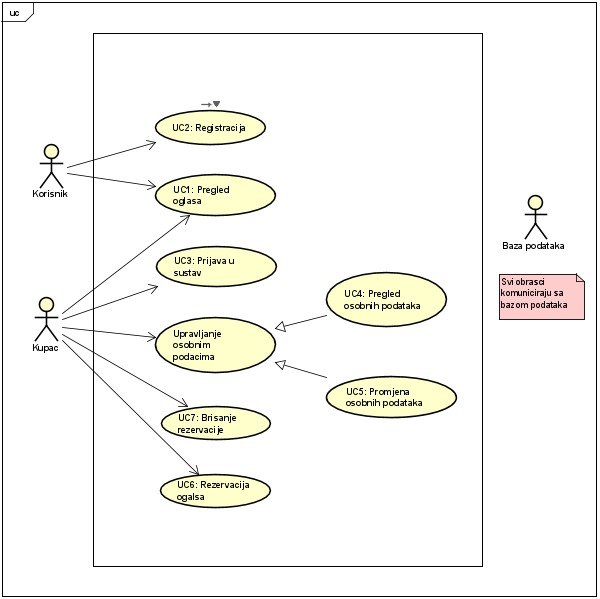
\includegraphics[scale=1]{dijagrami/DijagramOU1.PNG} %veličina slike u odnosu na originalnu datoteku i pozicija slike
						\centering
						\caption{ Dijagram obrasca uporabe, funkcionalnosti korisnika i kupca}
						\label{fig:dijagram1}
					\end{figure}
				
				
					\begin{figure}[H]
						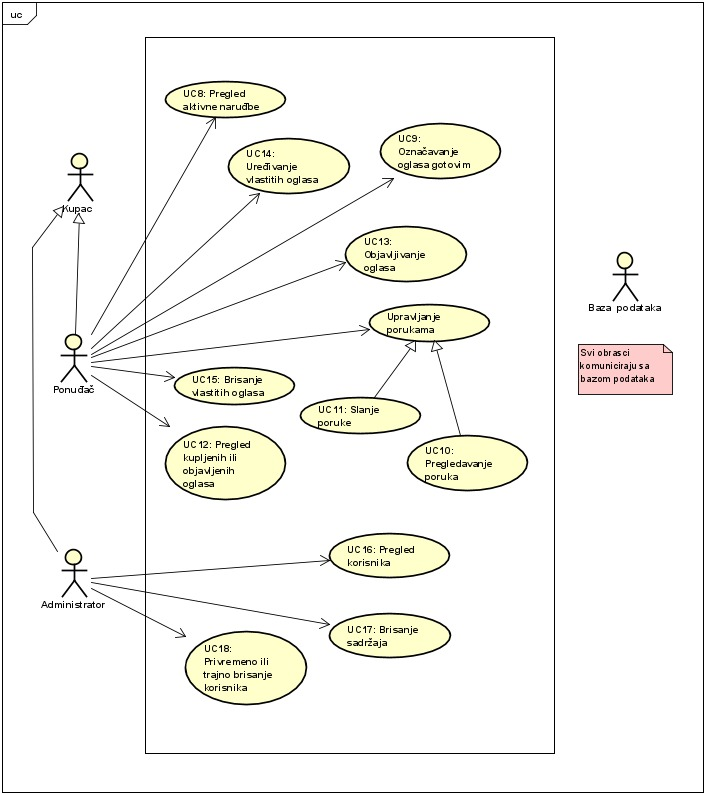
\includegraphics[scale=1]{dijagrami/DijagramOU2.PNG} %veličina slike u odnosu na originalnu datoteku i pozicija slike
						\centering
						\caption{ Dijagram obrasca uporabe, funkcionalnosti ponuđača i administratora}
						\label{fig:dijagram2}
					\end{figure}
				\eject		
				
			\subsection{Sekvencijski dijagrami}
				
				\textbf{UC6 - Rezervacija oglasa}

				Klijent salje zahtjev za prikaz svih oglasa. Posluzitelj dohvaca obliznje oglase i prikazuje ih. Odabirom oglasa,  posluzitelj iz baze podataka dohvaca osnovne podatke o oglasu i prikazuje ih korisniku. Da bi zapoceo rezervaciju, klijent salje zahtjev za rezervaciju. Posluzitelj u bazi podataka provjerava dostupnost oglasa. Ukoliko je oglas vec rezerviran, sustav obavjestava klijenta o tome uz poruku. Ako ogals nije rezerviran, posluzitelj informaciju o rezervaciji prosljeduje bazi koja sprema promjenu.
				
				\begin{figure}[H]
					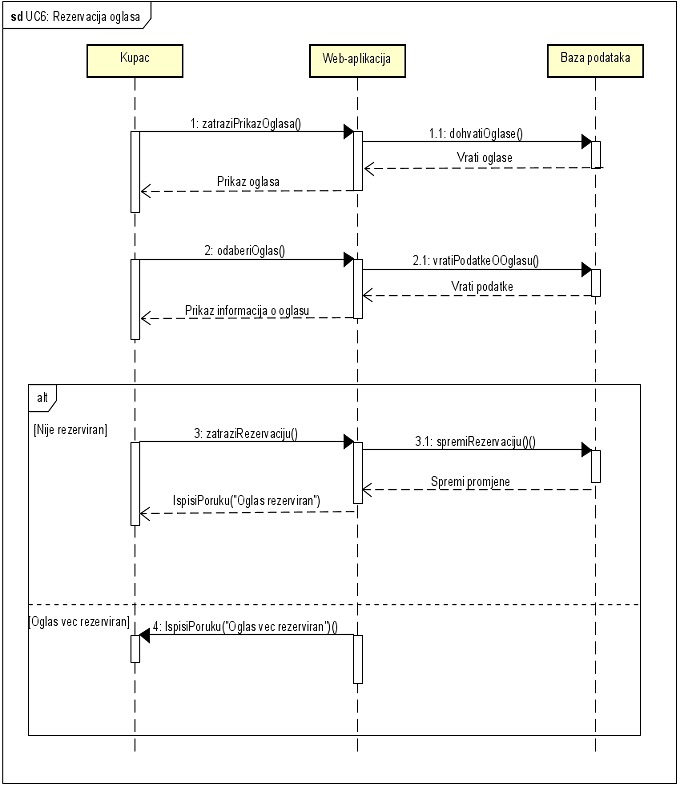
\includegraphics[scale=1]{dijagrami/SekvencijskiD.PNG} %veličina slike u odnosu na originalnu datoteku i pozicija slike
					\centering
					\caption{ Sekvencijski dijagram za UC6}
					\label{fig:dijagram3}
				\end{figure}
				\eject
	
		\section{Ostali zahtjevi}
		
		
			 
			 	\begin{itemize}
			 		\item Sustav treba omogućiti rad više korisnika u stvarnom vremenu
			 		
			 		\item Korisničko sučelje i sustav moraju podržavati hrvatsku abecedu (dijakritičke znakove) pri unosu i prikazu tekstualnog sadržaja
			 		
			 		
			 		\item  Izvršavanje dijela programa u kojem se pristupa bazi podataka ne smije trajati duže od nekoliko sekundi
			 		
			 		\item  Sustav treba biti implementiran kao web aplikacija koristeći objektno-orijentirane
			 		jezike
			 		
			 		\item  Neispravno korištenje korisničkog sučelja ne smije narušiti funkcionalnost i
			 		rad sustava
			 		
			 		\item  Sustav treba biti jednostavan za korištenje, korisnici se moraju znati koristiti
			 		sučeljem bez opširnih uputa
			 		
			 		\item  Nadogradnja sustava ne smije narušavati postojeće funkcionalnosti sustava
			 		
			 		\item  Sustav kao valutu koristi HRK
			 		
			 		\item  Veza s bazom podataka mora biti kvalitetno zaštićena, brza i otporna na vanjske greške
			 		
			 		\item  Pristup sustavu mora biti omogućen iz javne mreže pomoću HTTPS.
			 		
			 	\end{itemize}